\documentclass{article}
\usepackage{relsize}

\usepackage[utf8]{inputenc}
\usepackage{fancyhdr}
\usepackage{listings}
\usepackage{graphicx}
 
\pagestyle{fancy}
\fancyhf{}
\lhead{Exercise Sheet 3}
\rhead{Tim Schmiedl}
\rfoot{Page \thepage}

\begin{document}
\title{Data Analysis and Query Languages \\
 Exercise Sheet 3}
\date{\today}
\author{Tim Schmiedl} 
\maketitle

%%%%%%%%%%%%%%%%%%%%%%%%%%%%%%%%%%%%%%%%%%%%%%%%%%%%%%%%%%%%%
%%%%%%%%%%%%%%%%%%%%%%%%%%%%%%%%%%%%%%%%%%%%%%%%%%%%%%%%%%%%%
\section*{Exercise 1}
\lstinputlisting{ex3/ex1.txt} 


\vspace{2cm}
%%%%%%%%%%%%%%%%%%%%%%%%%%%%%%%%%%%%%%%%%%%%%%%%%%%%%%%%%%%%%
%%%%%%%%%%%%%%%%%%%%%%%%%%%%%%%%%%%%%%%%%%%%%%%%%%%%%%%%%%%%%
\section*{Exercise 2}
\subsection*{a) RDF Graph}
\begin{figure}[h!]
    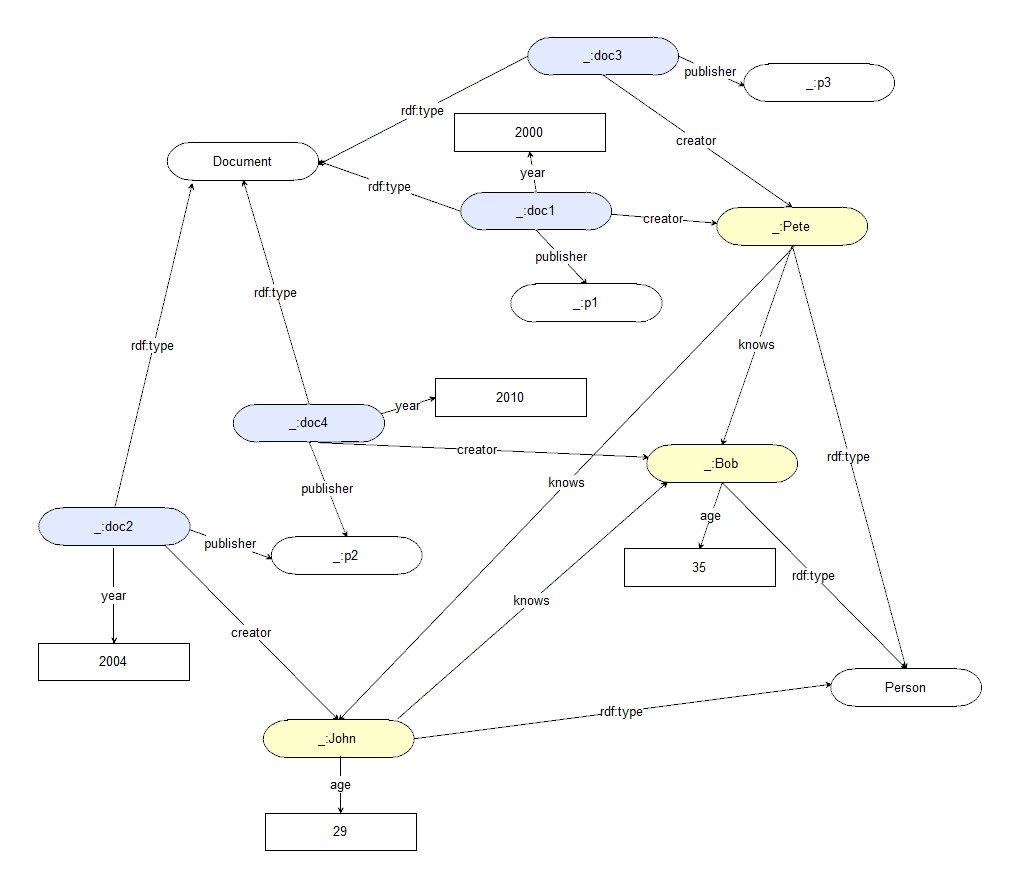
\includegraphics[width=1.2\textwidth]{img/rdf-graph.png}
\end{figure}

\subsection*{b) SPARQL}
\vspace{0.3cm}
(a) All Documents that are published after the year 2000.\\
\textbf{Result}: \{( :x, 2004), ( :y, 2010)\}\\
\vspace{0.3cm}

(b) All persons with an given age.\\
\textbf{Result}: \{( :x, 29), ( :y, 35), ( :z, )\}\\
\vspace{0.3cm}

(c) Persons for which an age is given or are the creator of something.\\
\textbf{Result}: \{( :x, 29, ), ( :y, 35, ), ( :z, , :a), ( :z, , :b), ( :x, ,
:c), ( :y, , :d)\}
\vspace{0.3cm}

\vspace{2cm}
%%%%%%%%%%%%%%%%%%%%%%%%%%%%%%%%%%%%%%%%%%%%%%%%%%%%%%%%%%%%%
%%%%%%%%%%%%%%%%%%%%%%%%%%%%%%%%%%%%%%%%%%%%%%%%%%%%%%%%%%%%%
\section*{Exercise 3}
\subsection*{a)}
\begin{lstlisting}
SELECT * WHERE {
	?p rdf:type myns:Person .
	?d1 rdf:type myns:Document .
	?d2 rdf:type myns:Document .
	?d1 myns:creator ?p.
	?d2 myns:creator ?p.
	
	Filter (?d1 != ?d2)
}

SELECT ?doc
WHERE
{
	?doc rdf:type myns:Document.
	?doc myns:creator ?creator
}
\end{lstlisting}

\subsection*{b)}
\begin{lstlisting}


\end{lstlisting}

\subsection*{c)}
\begin{lstlisting}
SELECT ?pub ?age
WHERE
{
	?doc myns:publisher ?pub.
	?doc myns:creator ?creator.

	OPTIONAL{ ?doc myns:year ?date.}
	OPTIONAL{ ?creator myns:age ?age .}
	
	FILTER(!bound(?date))
}
\end{lstlisting}


\vspace{2cm}
%%%%%%%%%%%%%%%%%%%%%%%%%%%%%%%%%%%%%%%%%%%%%%%%%%%%%%%%%%%%%
%%%%%%%%%%%%%%%%%%%%%%%%%%%%%%%%%%%%%%%%%%%%%%%%%%%%%%%%%%%%%
\section*{Exercise 4}



\end{document}
